\documentclass{article}

\usepackage{texmaths-main}
\usepackage{enumitem}
\usepackage{geometry}

\newgeometry{
        includehead,
        lmargin=50pt,
        textwidth=500pt,
        top=10pt%
        }

\long\def\newfig#1#2{%
\begin{minipage}[t]{.5\linewidth}
    #1\vskip20pt{\bfseries\Large Figure #2}
\end{minipage}%
\begin{minipage}[t]{.5\linewidth}
    \begin{tikzpicture}[scale=1.75]
        \draw(-2,-2)rectangle(2,2);
    \end{tikzpicture}
\end{minipage}\vskip20pt
}
\pagestyle{empty}
\begin{document}
Reproduire les figures de gauche dans le carré de droite.\vskip20pt
%---------
\newfig{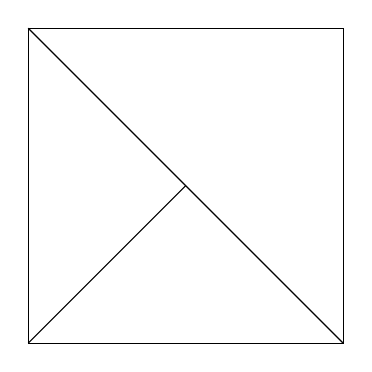
\begin{tikzpicture}
    \draw(-2,-2)rectangle(2,2);
    \draw(-2,2)--(2,-2);
    \draw(-2,-2)--(0,0);
\end{tikzpicture}}1\kern100pt
\newfig{%
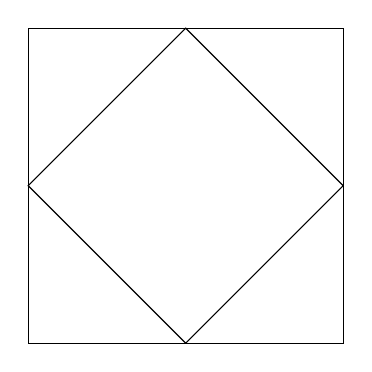
\begin{tikzpicture}
    \draw(-2,-2)rectangle(2,2);
    \draw(2,0)--(0,2)--(-2,0)--(0,-2)--cycle;
\end{tikzpicture}}2
% -----------------------
\newpage
\newfig{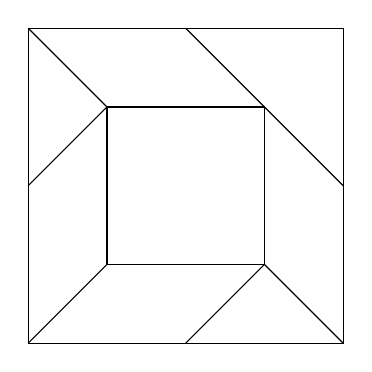
\begin{tikzpicture}
    \draw(-2,-2)rectangle(2,2);
    \draw(-1,-1)rectangle(1,1);
    \draw(-2,2)--(-1,1)--(-2,0);
    \draw(-1,-1)--(-2,-2);
    \draw(2,-2)--(1,-1)--(0,-2);
    \draw(0,2)--(2,0);
\end{tikzpicture}}3\kern100pt
\newfig{%
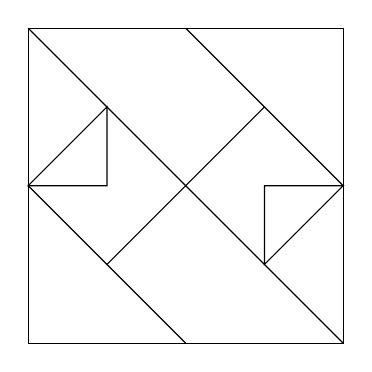
\begin{tikzpicture}
    \draw(-2,-2)rectangle(2,2);
    \draw(-2,2)--(2,-2);
    \draw(0,2)--(2,0);
    \draw(-2,0)--(0,-2);
    \draw(-1,-1)--(1,1);
    \draw(-2,0)--(-1,0)--(-1,1)--cycle;
    \draw(1,0)--(2,0)--(1,-1)--cycle;
\end{tikzpicture}}4\newpage
\newfig{\begin{tikzpicture}
    \draw(-2,-2)rectangle(2,2);
    \draw(-2,0)--(-1,0)--(-1,-1)--(1,-1)--(1,1)--(0,1)--(0,2);
    \draw(1,-1)--(2,-2);
\end{tikzpicture}}5\kern100pt
\newfig{%
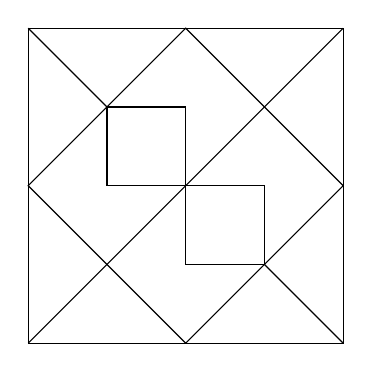
\begin{tikzpicture}
    \draw(-2,-2)rectangle(2,2);
    \draw(2,0)--(0,2)--(-2,0)--(0,-2)--cycle;
    \draw(-2,-2)--(2,2);
    \draw(-2,2)--(-1,1);
    \draw(1,-1)--(2,-2);
    \draw(-1,0)rectangle(0,1);
    \draw(0,0)rectangle(1,-1);
\end{tikzpicture}}6

\end{document}
